%----------------------------------------------------------------------------
%------------------------------Broad objectives------------------------------
%----------------------------------------------------------------------------
This chapter presents the main points from two basic studies: the equations of motion describing the interaction of the laser field and the target system are developed, and the connection between this research and the LIDAR remote sensing problem (see Figure \ref{general LIDAR}) is established.
%----------------------------------------------------------------------------
%----------------------------------------------------------------------------
%bb defines the bounding box for the pdf
%viewport defines the area of the pdf used
%in sidewaysfigure the last entry in bb moves the caption toward/away the pic
%in sidewaysfigure the second entry in bb moves the pic toward/away the caption
%----------------------------------------------------------------------------
\begin{figure}
\scalebox{0.6}[0.6]{
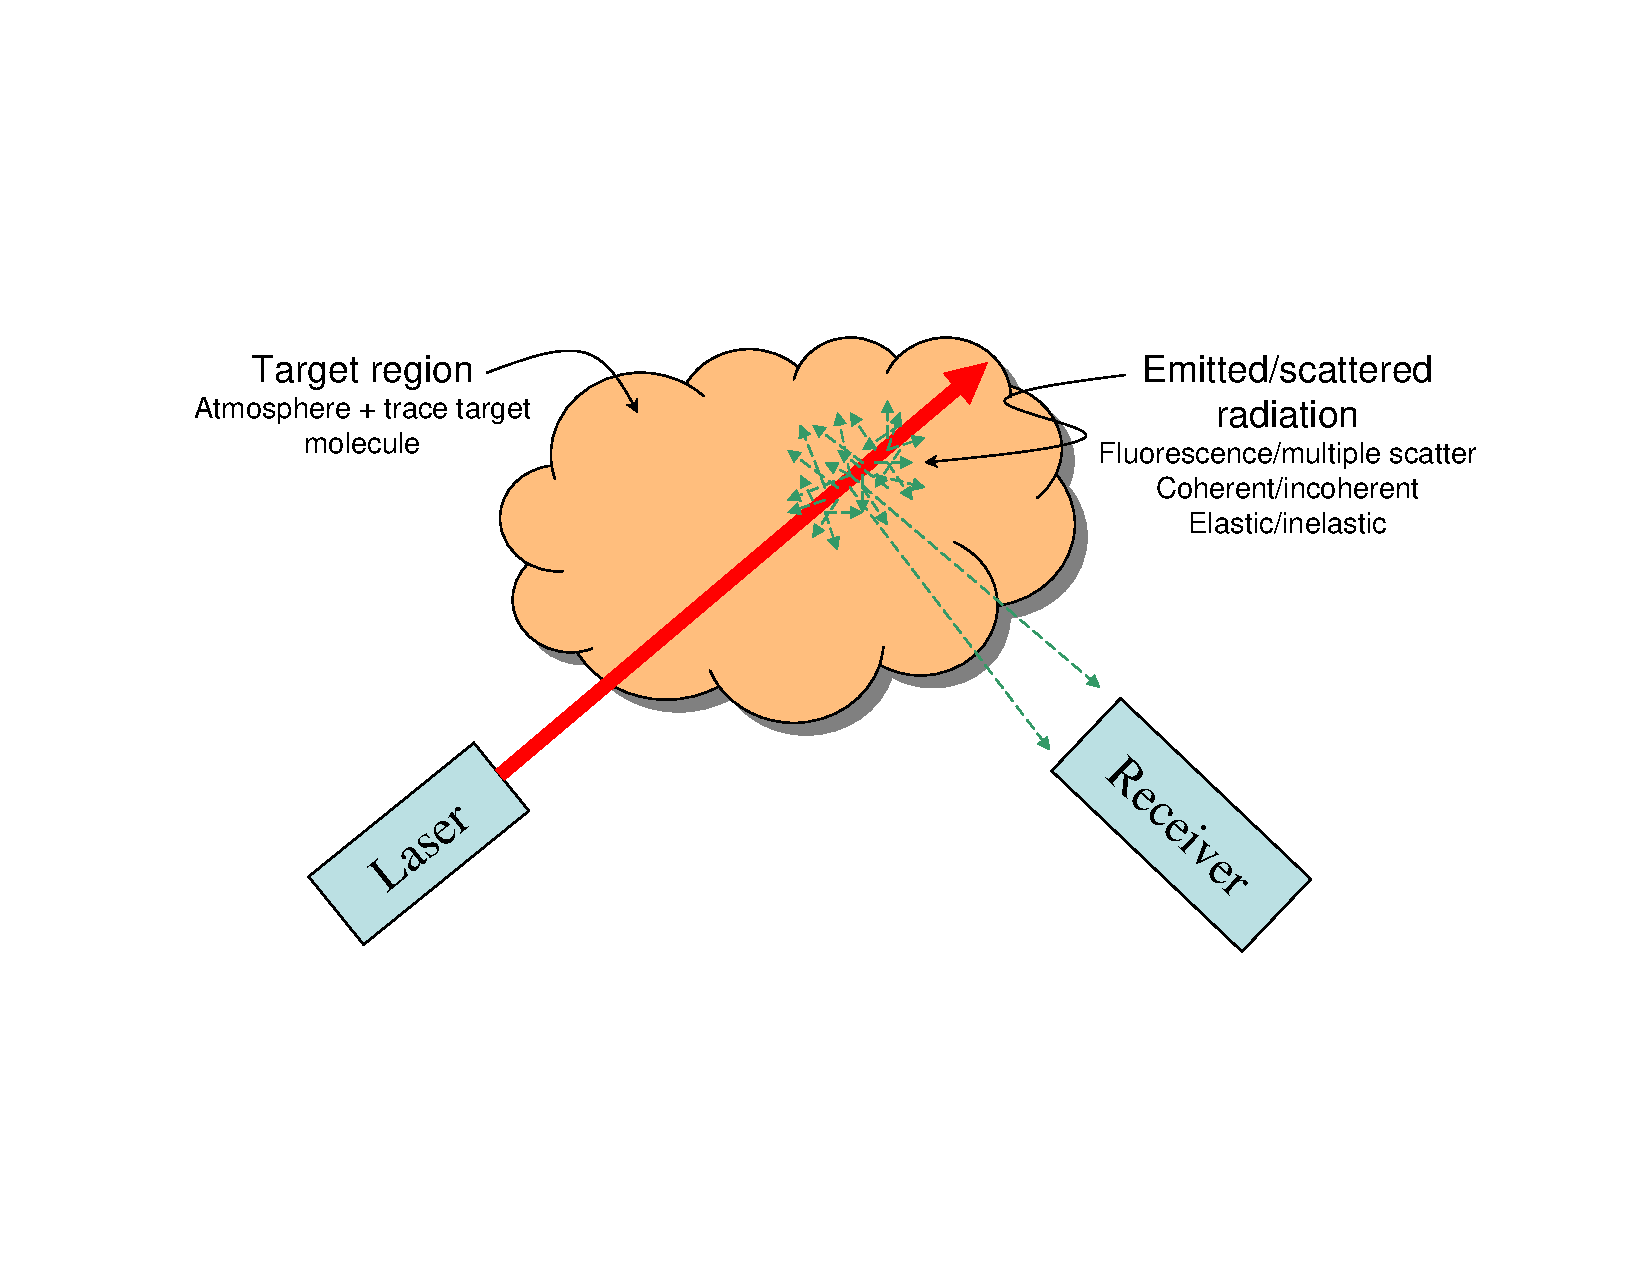
\includegraphics[bb=40 150 489 500]
{general_LIDAR/general_LIDAR.pdf}
}
\caption[General LIDAR schematic]{General remote sensing LIDAR schematic. A laser beam is used to excite a region of atmosphere while a receiver (telescope) collects the resulting emitted/scattered radiation. The spectral and temporal features of the acquired signal are used to determine the relative abundance of specific trace molecules.}
\label{general LIDAR}
\end{figure}
%----------------------------------------------------------------------------

%----------------------------------------------------------------------------
%----------------------------------------------------------------------------
%-------------------------concepts/results presented-------------------------
%----------------------------------------------------------------------------
We analyze the impact of random molecular \emph{classical} orientation and the thermal distribution of molecular velocities on the average observed behavior in LIF benchtop experiments; and the fundamental limits of LIDAR systems are explored using simple geometric and phase space arguments.
%----------------------------------------------------------------------------
%------------------relevant concepts/results NOT presented-------------------
%----------------------------------------------------------------------------

This is an idealized introduction. Many details are ignored to clarify the arguments. The formalism is very simplified and will be revisited in later chapters. In the phase space analysis of LIDAR systems, details of the detection process are ignored. The only detector feature preserved is the finite phase space available to the receiver. The acceptance phase space of the Interactive Technologies CT--103 1 m monochromator is used as a prototype and is by no means optimal (integrating spheres and atomic/molecular detection methods could increase the phase space available to the receiver). In an actual deployable system, a full analysis along the lines of the methods used in reference \cite{Lienert:2005a} should be used.
%----------------------------------------------------------------------------
%----------------------------------------------------------------------------
%----------------------------------------------------------------------------

Many introductory texts \cite{Louisell:1960a,Yariv:1989a,Bransden:1989a,Scully:1997a} outline the methods and assumptions used here to derive the equations of motion. These results are used to derive the average behavior of a randomly oriented ensemble. Reference \cite{Serway:1990a} gives the well known expression for the Maxwell-Boltzmann speed distribution from the kinetic theory of gases. This distribution is used to model the effects of the random motion of the target molecules on observed intensity fluctuations. Reference \cite{Hassani:1999a} describes the Liouville Theorem and reference \cite{Saleh:1991a} describes the ``ABCD'' matrix method of ray tracing which were both used to find the optimal lens combination of the receiver in the bench top experiment.
%----------------------------------------------------------------------------
%----------------------------------------------------------------------------
